\documentclass[a4paper, 12pt]{article}

% \usepackage[portuges]{babel}
\usepackage[utf8]{inputenc}
\usepackage{subfig}
\usepackage[colorinlistoftodos]{todonotes}

\usepackage[english]{babel}
\usepackage{indentfirst,setspace,subcaption}
\usepackage{amsmath,amssymb,graphicx,xcolor,url}
\usepackage{fancyhdr,tocbasic,titlesec,minted,listings}
\usepackage[a4paper,margin=24mm]{geometry}
\usepackage[skip=10pt plus1pt, indent=20pt]{parskip}
\usepackage[colorlinks=true,allcolors=blue,urlcolor=magenta]{hyperref}

\usepackage{indentfirst}
\usepackage{verbatim}
\usepackage{textcomp}
\usepackage{gensymb}
\usepackage{tabularx}
\usepackage{relsize}

\usepackage{lipsum}
\usepackage{xcolor}
\usepackage{xparse}
\NewDocumentCommand{\myrule}{O{1pt} O{2pt} O{black}}{%
  \par\nobreak%
  \kern\the\prevdepth%
  \kern#2
  {\color{#3}\hrule height #1 width\hsize}
  \kern#2
  \nointerlineskip%
}
\usepackage[section]{placeins}

\usepackage{booktabs}
\usepackage{colortbl}%
   \newcommand{\myrowcolour}{\rowcolor[gray]{0.925}}
   

\pagestyle{fancy}
\setlength{\headheight}{15pt}
\fancyhf{}
\fancyhead[R]{\nouppercase\rightmark\hfill~Exercise 2 Report}
\fancyfoot[C]{\hfill\thepage\hfill}

\DeclareTOCStyleEntry[
  indent=12pt,
  level=1
]{largetocline}{section}

\setlength{\marginparwidth}{2cm} 
\begin{document}

\begin{titlepage}
	\begin{center}
		\textbf{\LARGE Vietnam National University,}\\[0.5cm]
		\textbf{\LARGE Ho Chi Minh City}\\[0.5cm]
		\vspace{20pt}
		\textbf{\large UNIVERSITY OF SCIENCE}\\[0.2cm]
		\textbf{\large FACULTY OF INFORMATION TECHNOLOGY}\\[0.2cm]
		\vspace{20pt}
		
\includegraphics[width=0.5\textwidth,keepaspectratio]{./images/logo.png}

		\par
		\vspace{20pt}
		\textbf{\Large [CSC10004] Data Structure And Algorithms}\\
		\vspace{15pt}
		\myrule[1pt][7pt]
		\textbf{\LARGE EXERCISE 2 REPORT}\\
		\vspace{15pt}
		\textbf{\large Implementing Hash Table from scratch}\\
		\vspace{10pt}
		\myrule[1pt][7pt]
		\vspace{25pt}
		\textbf{\large Student Name \hspace{20pt} Student ID}\\
		Bui Minh Duy \hspace{45pt} 23127040 \\

		\vspace{45pt}
		\textbf {\large Lecturer In Charge}\\[0.2cm]
		\Large {Bui Duy Dang}\\[0.1cm]
		\Large {Nguyen Thanh Tinh}\\[0.1cm]
	\end{center}

	\par
	\vfill
	\begin{center}
		\text{17/08/2024}\\
	\end{center}

\end{titlepage}

\tableofcontents\thispagestyle{empty}

\pagebreak

\section{Student Information}
\begin{itemize}
	\item \textbf{Student ID:} 23127040
	\item \textbf{Full Name:} Bui Minh Duy
	\item \textbf{Class:} 23CLC09
\end{itemize}
\section{How I implemented the requirements}
\begin{itemize}
	\item At first, when implemented these hash tables, I found that in some specific cases, the hash table is not full but the insertion operation is failed. This is because the hash table is not rehashed when the load factor is greater than 0.5. Therefore, I have added the rehashing operation to the insertion operation.
	\item For the chaining using AVL tree, I have implemented the AVL tree from scratch. The AVL tree is a self-balancing binary search tree, so it is more efficient than the linked list in terms of searching and inserting operations. However, the AVL tree is much more complex than the linked list, so the AVL tree is slower than the linked list in terms of inserting operation.
	\item On dealing with string keys, I have used a specific hash function based on the hint in the requirements.
\end{itemize}
\section{Detailed Experiments}
\subsection{Operations}
\subsubsection*{Linear Probing}
\begin{figure}[H]
	\centering
	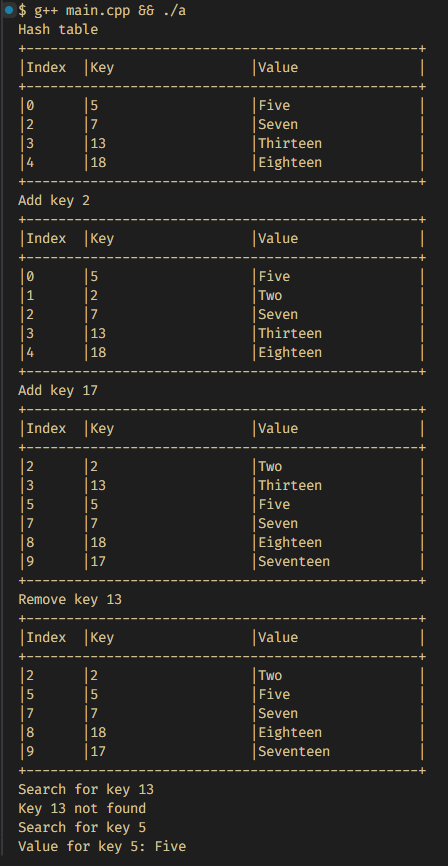
\includegraphics[width=0.5\textwidth, height=0.65\textheight]{images/linear_prob/main.png}
	\caption{Linear Probing Operations}
\end{figure}
\textbf{The hash table is initialized with size 5. Then, the following operations are performed:}
\begin{itemize}
	\item First, four keys \{7, 13, 5, 18\} are inserted to the hash table respectively.
	\item Then, key 2 is inserted (so the hash table becomes full).
	\item Continue inserting key 17 into the hash table (now the hash table needs to be rehashed to add key 17 successfully, and the indices have been changed).
	\item After that, key 13 is removed from the hash table.
	\item Therefore, when performing the search operation for key 13, it is not found in the hash table.
	\item However, key 5 is found in the hash table.
	\item Finally, the hash table is released and the program is terminated.
\end{itemize}

\subsubsection*{Quadratic Probing}
\begin{figure}[H]
	\centering
	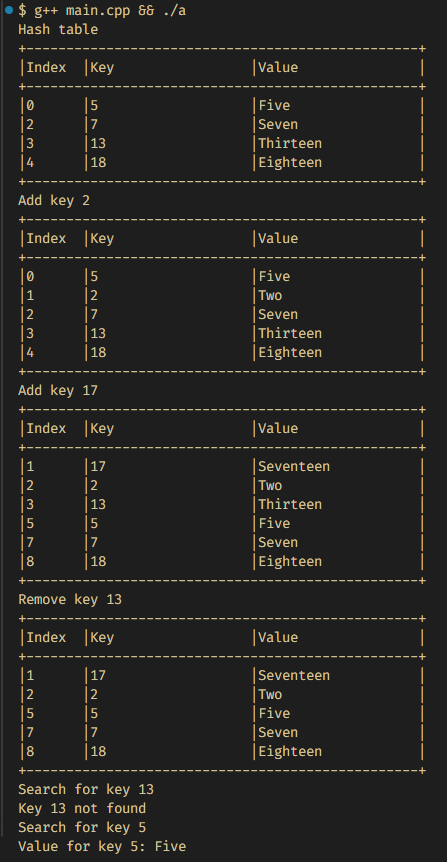
\includegraphics[width=0.5\textwidth, height=0.65\textheight]{images/quadratic_prob/main.png}
	\caption{Quadratic Probing Operations}
\end{figure}
\textbf{The hash table is initialized with size 5. Then, the following operations are performed:}
\begin{itemize}
	\item First, four keys \{7, 13, 5, 18\} are inserted to the hash table respectively.
	\item Then, key 2 is inserted (so the hash table becomes full).
	\item Continue inserting key 17 into the hash table (now the hash table needs to be rehashed to add key 17 successfully, and the indices have been changed).
	\item After that, key 13 is removed from the hash table.
	\item Therefore, when performing the search operation for key 13, it is not found in the hash table.
	\item However, key 5 is found in the hash table.
	\item Finally, the hash table is released and the program is terminated.
\end{itemize}

\subsubsection*{Chaining using Linked List}
\begin{figure}[H]
	\centering
	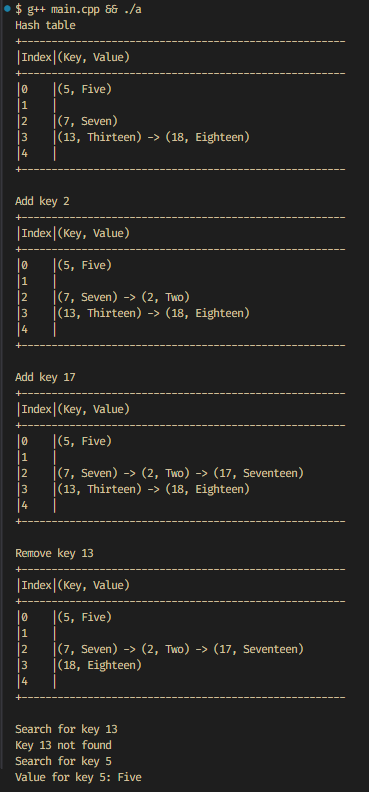
\includegraphics[width=0.5\textwidth, height=0.65\textheight]{images/chaining_ll/main.png}
	\caption{Chaining using Linked List Operations}
\end{figure}
\textbf{The hash table is initialized with size 5. Then, the following operations are performed:}
\begin{itemize}
	\item First, four keys \{7, 13, 5, 18\} are inserted to the hash table respectively.
	\item Then, key 2 and 7 are inserted.
	\item After that, key 13 is removed from the hash table.
	\item Therefore, when performing the search operation for key 13, it is not found in the hash table.
	\item However, key 5 is found in the hash table.
	\item Finally, the hash table is released and the program is terminated.
\end{itemize}

\subsubsection*{Chaining using AVL Tree}
\begin{figure}[H]
	\centering
	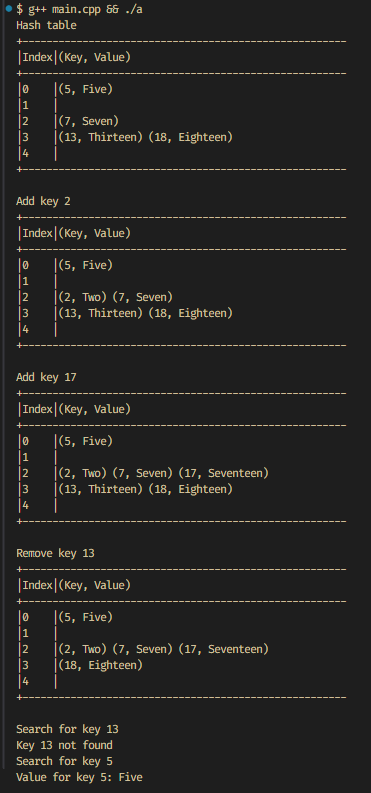
\includegraphics[width=0.5\textwidth, height=0.65\textheight]{images/chaining_avl/main.png}
	\caption{Chaining using AVL Tree Operations}
\end{figure}
\textbf{The hash table is initialized with size 5. Then, the following operations are performed:}
\begin{itemize}
	\item First, four keys \{7, 13, 5, 18\} are inserted to the hash table respectively.
	\item Then, key 2 and 7 are inserted.
	\item After that, key 13 is removed from the hash table.
	\item Therefore, when performing the search operation for key 13, it is not found in the hash table.
	\item However, key 5 is found in the hash table.
	\item Finally, the hash table is released and the program is terminated.
\end{itemize}

\subsubsection*{Double Hashing}
\begin{figure}[H]
	\centering
	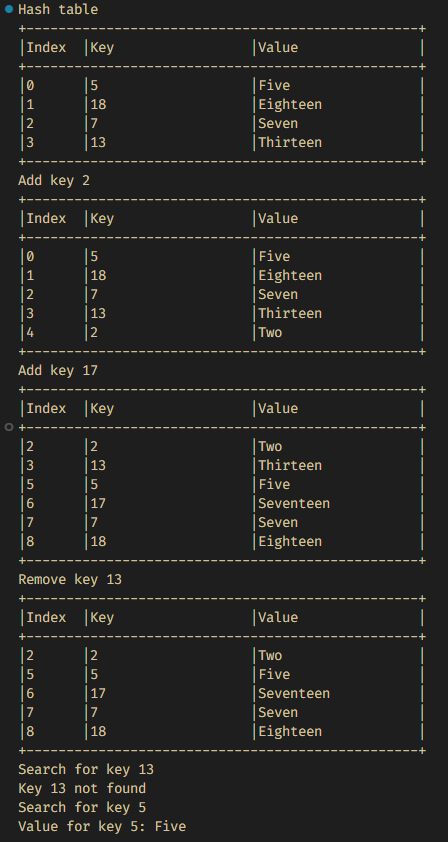
\includegraphics[width=0.5\textwidth, height=0.65\textheight]{images/double_hash/main.png}
	\caption{Double Hashing Operations}
\end{figure}
\textbf{The hash table is initialized with size 5. Then, the following operations are performed:}
\begin{itemize}
	\item First, four keys \{7, 13, 5, 18\} are inserted to the hash table respectively.
	\item Then, key 2 is inserted (so the hash table becomes full).
	\item Continue inserting key 17 into the hash table (now the hash table needs to be rehashed to add key 17 successfully, and the indices have been changed).
	\item After that, key 13 is removed from the hash table.
	\item Therefore, when performing the search operation for key 13, it is not found in the hash table.
	\item However, key 5 is found in the hash table.
	\item Finally, the hash table is released and the program is terminated.
\end{itemize}

\subsection{Performance}
\subsubsection*{Linear Probing}
\begin{figure}[H]
	\centering
	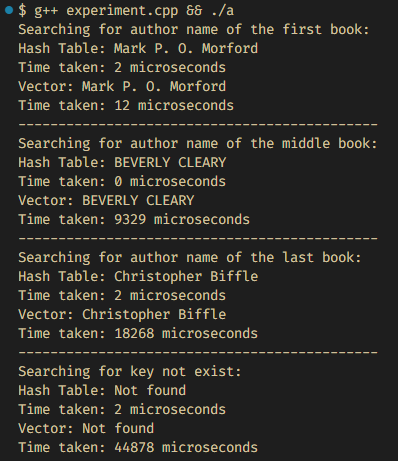
\includegraphics[width=0.6\textwidth]{images/linear_prob/experiment.png}
	\caption{Linear Probing Performance}
\end{figure}
\begin{itemize}
	\item Time Complexity of Linear Probing Search: \(O(n)\)
	\item Time Complexity of Linear Seach Algorithm: \(O(n)\)
\end{itemize}
Though having the same theorectical time complexity, the actual time execution of Linear Probing Search is much faster than Linear Search Algorithm, especially in the worst case.

\subsubsection*{Quadratic Probing}
\begin{figure}[H]
	\centering
	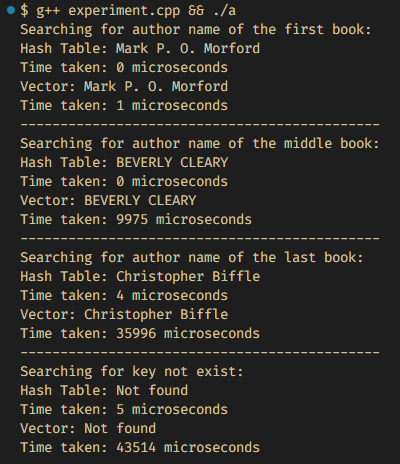
\includegraphics[width=0.6\textwidth]{images/quadratic_prob/experiment.png}
	\caption{Quadratic Probing Performance}
\end{figure}
\begin{itemize}
	\item Time Complexity of Quadratic Probing Search: \(O(n)\)
	\item Time Complexity of Linear Seach Algorithm: \(O(n)\)
\end{itemize}
Though having the same theorectical time complexity, the actual time execution of Quadratic Probing Search is much faster than Linear Search Algorithm, especially in the worst case.

\subsubsection*{Chaining using Linked List}
\begin{figure}[H]
	\centering
	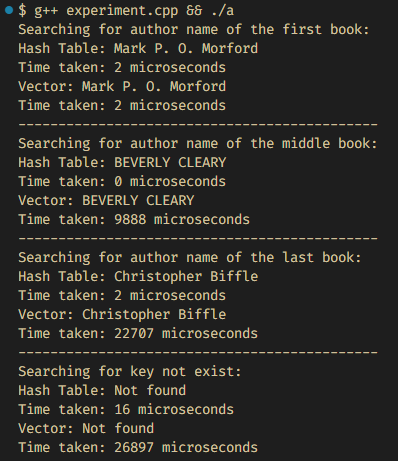
\includegraphics[width=0.6\textwidth]{images/chaining_ll/experiment.png}
	\caption{Chaining using Linked List Performance}
\end{figure}
\begin{itemize}
	\item Time Complexity of Chaining Search using Linked List: \(O(n)\)
	\item Time Complexity of Linear Seach Algorithm: \(O(n)\)
\end{itemize}
Though having the same theorectical time complexity, the actual time execution of Chaining Search using Linked List is much faster than Linear Search Algorithm, especially in the worst case.

\subsubsection*{Chaining using AVL Tree}
\begin{figure}[H]
	\centering
	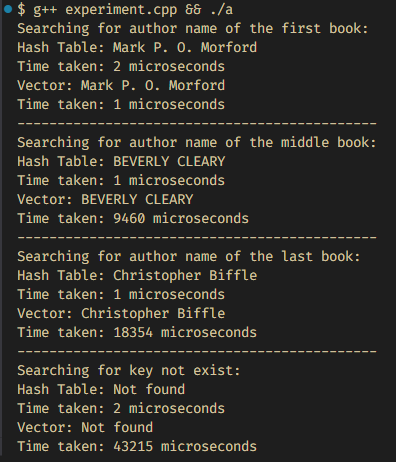
\includegraphics[width=0.6\textwidth]{images/chaining_avl/experiment.png}
	\caption{Chaining using AVL Tree Performance}
\end{figure}
\begin{itemize}
	\item Time Complexity of Chaining Search using AVL Tree: \(O(\log n)\)
	\item Time Complexity of Linear Seach Algorithm: \(O(n)\)
\end{itemize}
Chaining Search using AVL Tree has a better time complexity than Linear Search Algorithm in theorectical, and the actual time also proves that.

\subsubsection*{Double Hashing}
\begin{figure}[H]
	\centering
	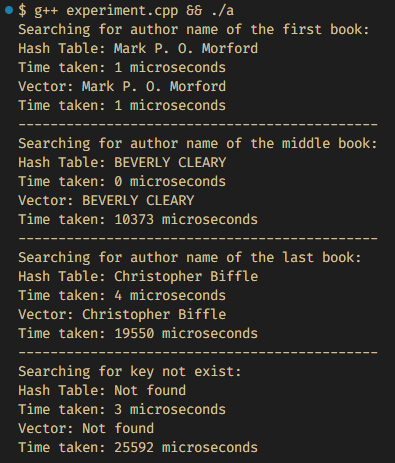
\includegraphics[width=0.6\textwidth]{images/double_hash/experiment.png}
	\caption{Double Hashing Performance}
\end{figure}
\begin{itemize}
	\item Time Complexity of Double Hashing Search: \(O(n)\)
	\item Time Complexity of Linear Seach Algorithm: \(O(n)\)
\end{itemize}
Though having the same theorectical time complexity, the actual time execution of Double Hashing Search is much faster than Linear Search Algorithm, especially in the worst case.

\section{Self-Evaluation}
\begin{center}
	\begin{tabularx}{0.7\textwidth}{|c|X|c|}
		\hline
		\textbf{No.} & \textbf{Details}           & \textbf{Score} \\ \hline
		1            & Linear Probing             & 100\%          \\ \hline
		2            & Quadratic Probing          & 100\%          \\ \hline
		3            & Chaining using Linked List & 100\%          \\ \hline
		4            & Chaining using AVL Tree    & 100\%          \\ \hline
		5            & Double Hashing             & 100\%          \\ \hline
		6            & Experiments                & 100\%          \\ \hline
		7            & Report                     & 100\%          \\ \hline
		             & \textbf{Total}             & \textbf{100\%} \\ \hline
	\end{tabularx}
\end{center}
\section{Exercise Feedback}
\subsection*{What I learned}
\begin{itemize}
	\item An thorough understanding of the concept of Hashing and its applications.
	\item Different types of Hashing techniques and their implementations.
	\item The application of AVL Tree in Hashing.
\end{itemize}

\subsection*{What I found challenging}
\begin{itemize}
	\item At first, the implementation of AVL Tree in Hashing was quite difficult and complex. However, after many attempts, I was able to understand the concept and method clearly and implement it successfully.
\end{itemize}
\section{References}
\begin{itemize}
	\item \href{https://www.geeksforgeeks.org/introduction-to-avl-tree/}{AVL Tree Data Structure} by GeeksforGeeks.
	\item \href{https://gvpress.com/journals/IJHIT/vol8_no3/18.pdf} {A Hybrid Chaining Model with AVL and Binary Search Tree to Enhance Search Speed in Hashing} by International Journal of Hybrid Information Technology.
	\item GitHub Copilot.
\end{itemize}

\end{document}
